%% For double-blind review submission, w/o CCS and ACM Reference (max submission space)
\documentclass[acmsmall,review,anonymous]{acmart}\settopmatter{printfolios=true,printccs=false,printacmref=false}
%% For double-blind review submission, w/ CCS and ACM Reference
%\documentclass[acmsmall,review,anonymous]{acmart}\settopmatter{printfolios=true}
%% For single-blind review submission, w/o CCS and ACM Reference (max submission space)
%\documentclass[acmsmall,review]{acmart}\settopmatter{printfolios=true,printccs=false,printacmref=false}
%% For single-blind review submission, w/ CCS and ACM Reference
%\documentclass[acmsmall,review]{acmart}\settopmatter{printfolios=true}
%% For final camera-ready submission, w/ required CCS and ACM Reference
%\documentclass[acmsmall]{acmart}\settopmatter{}

%% Journal information
%% Supplied to authors by publisher for camera-ready submission;
%% use defaults for review submission.
\acmJournal{PACMPL}
\acmVolume{1}
\acmNumber{ICFP} % CONF = POPL or ICFP or OOPSLA
\acmArticle{1}
\acmYear{2018}
\acmMonth{1}
\acmDOI{}
\startPage{1}

%% Copyright information
%% Supplied to authors (based on authors' rights management selection;
%% see authors.acm.org) by publisher for camera-ready submission;
%% use 'none' for review submission.
\setcopyright{none}
%\setcopyright{acmcopyright}
%\setcopyright{acmlicensed}
%\setcopyright{rightsretained}
%\copyrightyear{2018}           %% If different from \acmYear

\bibliographystyle{ACM-Reference-Format}
%% Note: author/year citations are required for papers published as an
%% issue of PACMPL.
\citestyle{acmauthoryear}

%%%%%%%%%%%%%%%%%%%%%%%%%%%%%%%%%%%%%%%%%%%%%%%%%%%%%%%%%%%%%%%%%%%%%%
%% Note: Authors migrating a paper from PACMPL format to traditional
%% SIGPLAN proceedings format must update the '\documentclass' and
%% topmatter commands above; see 'acmart-sigplanproc-template.tex'.
%%%%%%%%%%%%%%%%%%%%%%%%%%%%%%%%%%%%%%%%%%%%%%%%%%%%%%%%%%%%%%%%%%%%%%

\usepackage{bookmark}
\usepackage{booktabs}
\usepackage{subcaption}
\usepackage[utf8]{inputenc}
\usepackage[T1]{fontenc}
\usepackage{xspace}

% Haskell code snippets and useful shortcuts
\usepackage{minted}
\setminted[haskell]{escapeinside=@@}
\newcommand{\hs}{\mintinline{haskell}}
\newcommand{\cmd}[1]{\textsf{\color[rgb]{0,0,0.5} #1}}
\newcommand{\teq}{\smaller $\sim$}
\newcommand{\ghci}{$\lambda$>}
\newcommand{\defeq}{\stackrel{\text{def}}{=}}
\newcommand{\std}[1]{{\color[rgb]{0,0.3,0} #1}}
\newcommand{\blk}[1]{{\color[rgb]{0,0,0} #1}}

% Questions and todos
\newcommand{\q}[2]{\textbf{\color{blue} Question #1:} #2}
\newcommand{\todo}[2]{\textbf{\color{red} #1:} #2}

% Abbreviations for build systems
\newcommand{\Make}{\textsc{Make}\xspace}
\newcommand{\Shake}{\textsc{Shake}\xspace}
\newcommand{\Ninja}{\textsc{Ninja}\xspace}
\newcommand{\Bazel}{\textsc{Bazel}\xspace}
\newcommand{\Buck}{\textsc{Buck}\xspace}
\newcommand{\Excel}{\textsc{Excel}\xspace}
\newcommand{\Calc}{\textsc{Calc}\xspace}

\begin{document}

%% [Short title] Title
\title[Build Systems \`a la Carte]{Build Systems \`a la Carte}
% \titlenote{with title note}
% \subtitle{Subtitle}
% \subtitlenote{with subtitle note}

%% Author information
%% Contents and number of authors suppressed with 'anonymous'.
%% Each author should be introduced by \author, followed by
%% \authornote (optional), \orcid (optional), \affiliation, and
%% \email.
%% An author may have multiple affiliations and/or emails; repeat the
%% appropriate command.
%% Many elements are not rendered, but should be provided for metadata
%% extraction tools.

%% Author with single affiliation.
\author{First1 Last1}
\authornote{with author1 note}          %% \authornote is optional;
                                        %% can be repeated if necessary
\orcid{nnnn-nnnn-nnnn-nnnn}             %% \orcid is optional
\affiliation{
  \position{Position1}
  \department{Department1}              %% \department is recommended
  \institution{Institution1}            %% \institution is required
  \streetaddress{Street1 Address1}
  \city{City1}
  \state{State1}
  \postcode{Post-Code1}
  \country{Country1}                    %% \country is recommended
}
\email{first1.last1@inst1.edu}          %% \email is recommended

%% Author with two affiliations and emails.
\author{First2 Last2}
\authornote{with author2 note}          %% \authornote is optional;
                                        %% can be repeated if necessary
\orcid{nnnn-nnnn-nnnn-nnnn}             %% \orcid is optional
\affiliation{
  \position{Position2a}
  \department{Department2a}             %% \department is recommended
  \institution{Institution2a}           %% \institution is required
  \streetaddress{Street2a Address2a}
  \city{City2a}
  \state{State2a}
  \postcode{Post-Code2a}
  \country{Country2a}                   %% \country is recommended
}
\email{first2.last2@inst2a.com}         %% \email is recommended
\affiliation{
  \position{Position2b}
  \department{Department2b}             %% \department is recommended
  \institution{Institution2b}           %% \institution is required
  \streetaddress{Street3b Address2b}
  \city{City2b}
  \state{State2b}
  \postcode{Post-Code2b}
  \country{Country2b}                   %% \country is recommended
}
\email{first2.last2@inst2b.org}         %% \email is recommended

\begin{abstract}
Build systems are awesome. Build systems are terrifying. In this paper ...
\end{abstract}

%% 2012 ACM Computing Classification System (CSS) concepts
%% Generate at 'http://dl.acm.org/ccs/ccs.cfm'.
\begin{CCSXML}
<ccs2012>
<concept>
<concept_id>10011007.10011006.10011008</concept_id>
<concept_desc>Software and its engineering~General programming languages</concept_desc>
<concept_significance>500</concept_significance>
</concept>
<concept>
<concept_id>10003456.10003457.10003521.10003525</concept_id>
<concept_desc>Social and professional topics~History of programming languages</concept_desc>
<concept_significance>300</concept_significance>
</concept>
</ccs2012>
\end{CCSXML}

\ccsdesc[500]{Software and its engineering~General programming languages}
\ccsdesc[300]{Social and professional topics~History of programming languages}
%% End of generated code

% \keywords{functional programming, build systems}

\maketitle

\section{Introduction}\label{sec-intro}

Build systems (such as \Make) are big, complicated, but unloved part of
the software ecosystem.  Every developer on the planet uses one, but
they are very much a means to an end, and seldom the focus of
attention.  But the challenges of scale have driven large software firms
like Microsoft, Facebook, and Google to develop their own build
systems, each with its own choices and idiosyncrasies.

Seldom do people ask questions like ``What does it mean for my build
system to be correct?'' or ``What are the trade-offs between different
approaches?''.  Complex build systems use subtle algorithms, but they
are often hidden away, and not the object of study.

In this paper we offer a general framework in which to discuss these
questions in a way that is both abstract (omitting incidental detail)
and yet precise (implemented as Haskell code).  Specifically we make
these contributions:
\begin{itemize}
\item We describe some simple but novel abstractions that
crisply encapsulate what a build system is.
\item We show that we can instantiate
these abstractions to describe the essence of a variety of different
build systems, including \Make, \Shake, \Bazel, and \Excel, each in
a dozen lines of code or so.
Doing this in a single setting allows
the differences and similarities between these huge systems to be
brought out clearly.
\item Build systems vary on many axes;
for example: static vs dynamic dependencies; cloud-build, including
shallow vs deep; deterministic vs non-deterministic build rules;
early cut-off; self-tracking build systems; and persistent metadata.
These properties (which we define in~\S\ref{sec-background}) are often
deeply-built-in assumptions of a particular build system.
In contrast, our framework allows them to be distinguished,
reasoned about, and varied.
\item Two particularly desirable properties are dynamic dependencies
and cloud-build; yet no currently-available build system supports
both.  Our framework makes it rather easy to do so, for the first
time.
\end{itemize}
Thus equipped, instead of seeing build systems as unrelated
points in space, we can re-envisage them as locations in a landscape,
leading to better understanding of what they do and how they compare,
and suggesting exploration of other (as yet unoccupied points) in the
landscape.

Papers about "frameworks" are often fuzzy.  This one is not: all our
abstractions are defined in Haskell, and we have (freely-available)
executable models of all the build systems we describe.  An unusual
feature is that we include \Excel in our line-up because, looked at
in the right way, it certainly is a build system.

\todo{AM/NM}{Add a paragraph on the decomposition of build systems into
\emph{compute} and \emph{build} components, with the latter split into
\emph{when} and \emph{how} parts.}

\clearpage
\section{Background}\label{sec-background}

Build systems automate the execution of simple repeatable tasks for individual
users, as well as for large organisations. There are software build systems,
such as \Make~\cite{feldman1979make}, \Shake~\cite{mitchell2012shake} and
\Bazel~\cite{bazel}, as well as various incremental calculation engines, such
as \Excel~\cite{advanced_excel}. In this section we use these four examples to
introduce main domain-specific notions and requirements. Other notable examples
of build systems and their relation to these four will be discussed
in~\S\ref{sec-related} and~\S\ref{sec-conclusions}.

\subsection{The venerable \Make: static dependencies and file modification times}
\label{sec-background-make}

\Make\footnote{There are numerous implementations of \Make and none comes with a
formal specification. In this paper we therefore use a simple and sensible
approximation to a real \Make that you might find on your machine.} was developed
more than 40 years ago to automatically build software libraries and executable
programs from source code. It uses \emph{makefiles} to describe build tasks and
their dependencies in a simple text form. For example:

\vspace{1mm}
\begin{minted}[xleftmargin=10pt]{makefile}
util.o: util.h util.c
    gcc -c util.c

main.o: util.h main.c
    gcc -c main.c

main.exe: util.o main.o
    gcc util.o main.o -o main.exe
\end{minted}
\vspace{1mm}

\noindent
The above makefile lists three tasks: (i) compile a utility library comprising
files \cmd{util.h} and \cmd{util.c} into \cmd{main.o} by
executing\footnote{In this example we treat \cmd{gcc} as a pure function for the
sake of simplicity. In reality there are multiple versions of \cmd{gcc} and the
actual binary that is used to compile and link files is also listed as a task
dependency.} the command \cmd{gcc -c util.c}, (ii) compile the main source file
\cmd{main.c} into \cmd{main.o}, and (iii) link object files \cmd{util.o} and
\cmd{main.o} into the executable \cmd{main.exe}. The makefile contains the
complete information about the \emph{task dependency graph}, which is shown in
Fig.~\ref{fig-make}(a).

\begin{figure}[h]
\begin{subfigure}[b]{0.32\linewidth}
\centerline{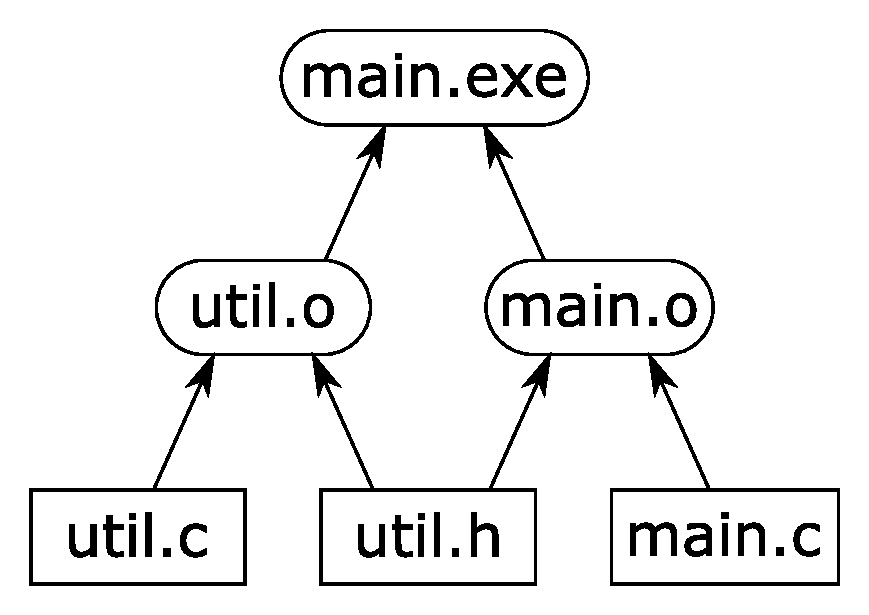
\includegraphics[scale=0.28]{fig/make-example.pdf}}
\caption{Task dependency graph}
\end{subfigure}
\begin{subfigure}[b]{0.32\linewidth}
\centerline{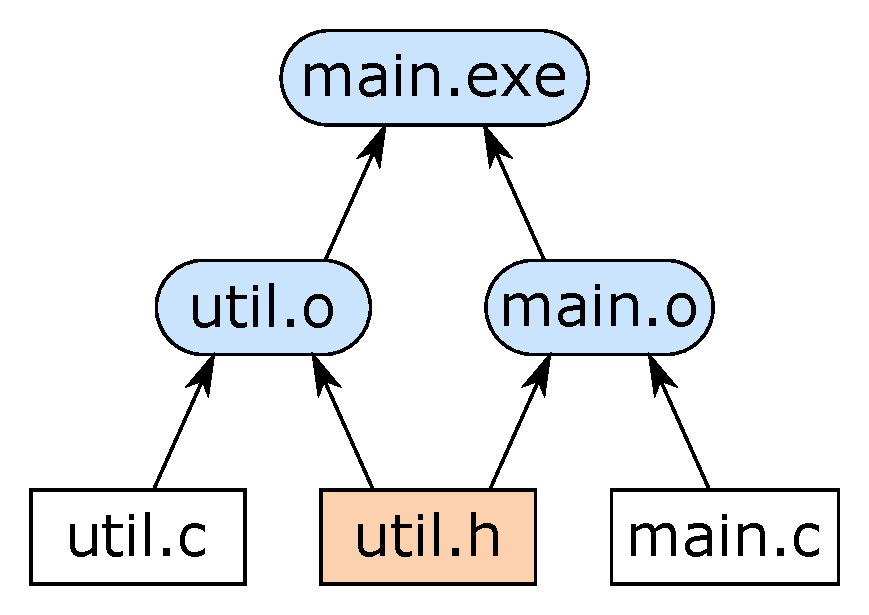
\includegraphics[scale=0.28]{fig/make-example-full.pdf}}
\caption{Full rebuild}
\end{subfigure}
\begin{subfigure}[b]{0.32\linewidth}
\centerline{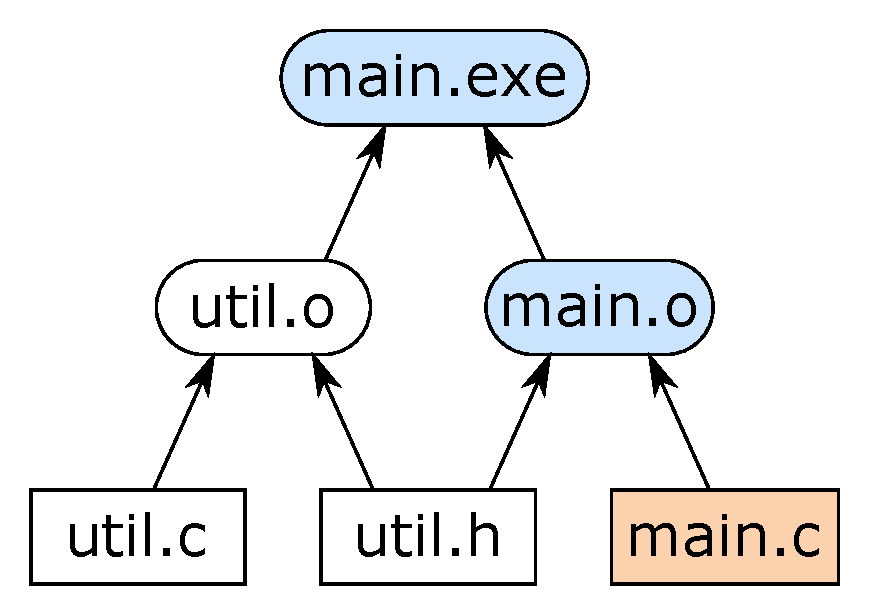
\includegraphics[scale=0.28]{fig/make-example-partial.pdf}}
\caption{Partial rebuild}
\end{subfigure}
\caption{A task dependency graph and two build scenarios. Input files are shown as
rectangles, intermediate and output files are shown as rounded rectangles. Dirty
inputs and files that are rebuilt are highlighted.
\label{fig-make}}
\end{figure}

If the user modifies the sources of the utility library and runs \Make, it will
perform a full rebuild, because all three tasks transitively depend on the
library, as illustrated in Fig.~\ref{fig-make}(b). On the other hand, if the
user modifies \cmd{main.c} then a partial rebuild is sufficient: indeed, the
file \cmd{util.o} does not need to be rebuilt, since its inputs have not
changed, see Fig.~\ref{fig-make}(c). Files that have changed since the previous
build are called \emph{dirty}.

The requirement to \emph{execute tasks at most once and only if they transitively
depend on dirty inputs} is essential for build systems, it is their raison
d'\^etre. We will call build systems that satisfy this requirement \emph{minimal}.

To achieve minimality \Make relies on two main ideas. First, it uses \emph{file
modification time} to detect the files that are dirty: a file is marked dirty if
it was modified since the previous build. Second, it constructs a complete task
dependency graph from the information contained in the makefile and executes
tasks in a \emph{topological order}.

Note that it is not always possible to know the dependencies of a task upfront,
or \emph{statically}. To demonstrate this, let us add another task to the above
makefile:

\vspace{1mm}
\begin{minted}[xleftmargin=10pt]{makefile}
release.tar: main.exe README
    tar -cf release.tar main.exe README
\end{minted}
\vspace{1mm}

\noindent
So far so good: if either \cmd{main.exe} or \cmd{README} is dirty, \Make will
recreate the release archive. But now imagine that we need to specify the files
that go into \cmd{release.tar} in a text file \cmd{release.txt}. The dependencies
of \cmd{release.tar} are no longer known statically: they \emph{depend on the
contents} of \cmd{release.txt}, which might not even exist before the build
starts, e.g. if it is produced by concatenating input files \cmd{release-bins.txt}
and \cmd{release-docs.txt}. Alas, makefiles cannot express such \emph{dynamic
dependencies}, requiring ad hoc workarounds such as \emph{build phases}, which
are problematic~\cite{hadrian}.

\subsection{\Excel: dynamic dependencies at the cost of minimality}
\label{sec-background-excel}

\Excel is a build system that can deal with dynamic dependencies albeit at the
cost of sacrificing minimality. Consider the following spreadsheet comprising
four input cells \cmd{A1-A3} and \cmd{B1}, and a single task computing the sum
of values \cmd{A1} $+\cdots+$ \cmd{An}, where \cmd{n} is specified indirectly in
\cmd{B1}:

\vspace{1mm}
\begin{minted}[xleftmargin=10pt]{bash}
A1 = 10
A2 = 20
A3 = 30
B1 = 2
C1 = SUM(A1:INDIRECT("A" & B1))
\end{minted}
\vspace{1mm}

\noindent
The output \cmd{C1} here is analogous to the \cmd{release.tar} from the previous
example: one cannot statically determine the dependencies of the associated task.
To deal with this, \Excel takes a simple conservative approach: it marks all
cells with dynamic dependencies as dirty and therefore always recomputes them
during a rebuild. This guarantees that the build result is correct, but clearly
violates the minimality requirement: if the user modifies \cmd{A3}, \Excel will
recompute \cmd{C1} even though it does not transitively depend on \cmd{A3}.

Note that \Excel's approach to marking cells as dirty is a relatively minor
variation of the approach used by \Make: a cell is considered dirty if it was
modified since the previous build \emph{or if it is volatile}, where the notion
of volatility includes dynamic dependencies, as well as \emph{non-determinism}
that will be discussed in~\S\ref{sec-engineering}. We therefore put both \Make
and \Excel in the same category of build systems that associate a \emph{dirty bit}
with every file or cell. (To avoid the ``file or cell'' nuisance, we introduce the
abstract notion of \emph{keys} in~\S\ref{sec-background-vocabulary}.)

\Excel's recalculation algorithm~\cite{excel_recalc} on the other hand is
significantly different from \Make. Since it is impossible to construct the full
dependency graph upfront in the presence of dynamic dependencies, \Excel
maintains the \emph{calculation chain}, which is an approximation to the correct
topological order. During recalculation, \Excel processes cells in this order,
but can \emph{defer recalculation of a cell} by moving it down the chain when newly
discovered dynamic dependencies dictate that. We discuss this algorithm in more
detail in~\S\ref{sec-examples}.

Another distinguishing feature of \Excel is \emph{self-tracking}. Most build
systems track changes of inputs and intermediate results, executing dependent
tasks whenever they change, but \Excel can also track changes in the tasks
themselves: if a formula is modified, \Excel will recompute it and propagate
the changes. Self-tracking is uncommon in software build systems, where one
often needs to manually initiate a full rebuild even if just a single task has
changed.

\subsection{\Shake: dynamic dependencies with no remorse}
\label{sec-background-shake}

\Shake was developed specifically to address the issue of dynamic
dependencies~\cite{mitchell2012shake} and it excels at handling them without
sacrificing the minimality requirement. Here is how one can express the task
for producing \cmd{release.tar} from the example discussed
in~\S\ref{sec-background-make}.

\vspace{1mm}
\begin{minted}[xleftmargin=10pt]{haskell}
"release.tar" %> \_ -> do
    need ["release.txt"]
    contents <- lines <$> readFile "release.txt"
    need contents
    system "tar" $ ["-cf", "result.tar"] ++ contents
\end{minted}
\vspace{1mm}

\noindent
We first declare the static dependency on \cmd{release.txt}, then read its
content and depend on it, dynamically. Finally, we specify the command to
produce the resulting archive. Crucially, the archive will only be rebuilt if
one of the dependencies (static or dynamic) has changed.

\todo{AM}{How is \Shake different.}

\begin{figure}[h]
\centerline{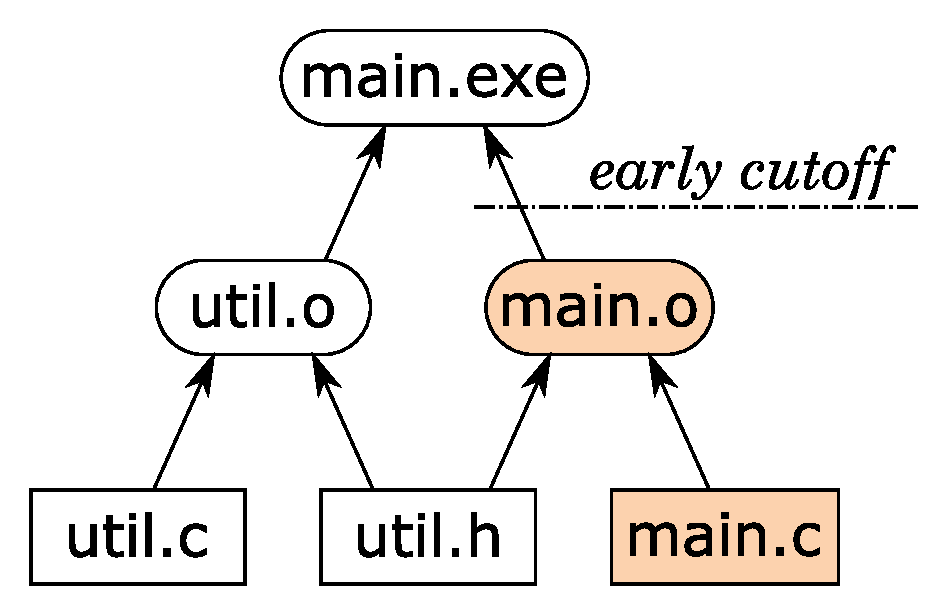
\includegraphics[scale=0.28]{fig/make-example-cutoff.pdf}}
\vspace{-2mm}
\caption{An early cutoff example: modify the source \cmd{main.c} by adding a
comment. The rebuild is stopped after detecting that \cmd{main.o} is unchanged,
which indicates that \cmd{main.exe} does not need to be rebuilt.\label{fig-cutoff}}
\end{figure}

\Shake also supports the following \emph{early cutoff optimisation}. When it
executes a task and the result is unchanged from the previous build, it is
unnecessary to execute the dependent tasks, and hence \Shake can stop a build
earlier, as illustrated in Fig.~\ref{fig-cutoff}. Not all build systems support
early cutoff: \Make and \Excel do not, whereas \Shake and \Bazel (introduced
below) do.

...

\subsection{\Bazel: a cloud build system}
\label{sec-background-shake}

When build systems are used by large teams, different team members
often end up executing exactly the same tasks on their local machines.
A \emph{cloud build system} can speed up builds dramatically by
transparently sharing build results among team members. Furthermore, cloud
build systems allow one to perform \emph{shallow builds} that materialise
only end build products on a local machine, leaving all intermediates in the
cloud. This is a significant optimisation compared to \emph{deep builds}
that require all transitive dependencies of an end build product to be
locally available. Non-cloud build systems cannot support shallow builds.

\subsection{Abstract vocabulary for build systems}
\label{sec-background-vocabulary}

\subsection{Keys, values, hashes and store}

Keys are
used to distinguish values. In build systems keys are typically filenames, e.g.
\cmd{main.c}, whereas values are file contents (a C program source code in this
case). In spreadsheets keys are cell names, e.g. \cmd{A1}, and values are
numbers, text, etc. that are typically displayed inside cells. In Haskell code,
we will use type variables \hs{k} and \hs{v} to denote keys and values,
respectively.


A \emph{store} associates keys to values. It is convenient to assume that a store
is total, i.e. it contains a value for every possible key. We therefore also
assume that the type of values is capable of encoding values corresponding to
non-existent keys (missing files or empty cells).

We use a cryptographic \emph{hash function} \hs{hash :: v -> Hash} for
efficient tracking and sharing of build results.

\subsection{Input, intermediate and output values}

Some values must be provided by the user as \emph{input}. For example,
\textsf{src/file.c} can be edited by the user who relies on the build system to
compile it into \textsf{obj/file.o}. Similarly, the user can input \textsf{A1 = 5}
and \textsf{B1 = 9} expecting the spreadsheet to compute their sum in \textsf{C1},
i.e. \textsf{C1 = 14}.

In the above examples, \textsf{obj/file.o} and \textsf{C1} are \emph{output} values.

In some situations we might also need the notion of \emph{intermediate} values,
which are not interesting for the user but are produced in the process of turning
inputs into outputs. For example, the user might only be interested in the
executable \textsf{bin/file.exe} obtained by linking \textsf{obj/file.o} with
standard libraries, in which case \textsf{obj/file.o} can be considered an
intermediate value.

\subsection{Non-deterministic computations}

Build systems and spreadsheets compute output values from input and intermediate
values. In the most typical case, these \emph{computations} are \emph{functions},
such as \textsf{C1 = A1 + B1}, i.e. their result is uniquely determined by the
input values. However, in general they can be \emph{relations}, i.e. have
multiple valid results. A spreadsheet example: \textsf{A2 = A1 + RANDOM(1,6)}.
This computation has six valid results for each input value \textsf{A1}. In
build systems, the object file \textsf{obj/file.o} is sometimes not uniquely
determined by the source \textsf{src/file.c} -- different compiler runs may
produce different valid results.


\begin{itemize}

    \item Some build systems, e.g. \Buck, require all tasks to be
    \emph{deterministic}, i.e. produce exactly the same output when run on the
    same inputs. However, not all tasks are deterministic, and there are build
    systems that support \emph{non-determinism}. A simple example is \Excel's
    \textsf{RANDBETWEEN(low, high)} that returns a random integer in the
    interval \textsf{[low, high]}.

    \item Most build systems persistently store auxiliary \emph{build
    information} for profiling and optimisation purposes: \Make stores file
    modification times, \Shake stores the discovered dynamic dependency graph,
    \Bazel and other cloud build systems store information about inputs and
    outputs of previously executed tasks, etc.
\end{itemize}

This paper presents a purely functional abstraction for build systems that
allows us to express all the above intricacies of build systems and design
complex build systems from simple primitives. The presented abstraction fits in
just two lines of Haskell code, which are explained
in~\S\ref{sec-abstractions}:

\begin{minted}{haskell}
type Compute c k v = @\std{forall}@ f. c f => (k -> f v) -> k -> Maybe (f v)
type Build c i k v = Compute c k v -> k -> Maybe i -> Map k v -> (i, Map k v)
\end{minted}


Below we define basic notions used in build systems and other similar domains,
for example, spreadsheets.


\subsection{Requirements for build systems}

\begin{itemize}
    \item Correctness
    \item Minimality
    \item Support for sharing and skipping intermediate values
\end{itemize}
...

\clearpage

\section{Build systems, abstractly}\label{sec-abstractions}

In this section we present the \emph{compute} and \emph{build} abstractions:
\begin{itemize}
    \item Compute represents build rules (in build systems) or formulas (in
    spreadsheets), and is completely isolated from the world of compilers, file
    systems, memories, caches, and all other complexities of real build systems.
    \item Build corresponds to the algorithm used for bringing a key-value store
    to a coherent state by running compute.
\end{itemize}

\begin{figure}
\begin{minted}{haskell}
type Compute c k v = @\std{forall}@ f. c f => (k -> f v) -> k -> Maybe (f v)
\end{minted}
\caption{Compute abstractions}\label{fig-compute}
\end{figure}

Consider abstractions in Fig.~\ref{fig-compute}.

...

We now describe several types of build systems according to their constraint
on the functor \hs{f}.

...


\clearpage
\section{Build systems, concretely}\label{sec-implementations}

In the previous sections we've discussed the types of build system in text, but the way we came to our conclusions was by developing a framework to fit the builds in. In this section we explain the framework, some of the abstractions we introduced (which model the properties from \S\ref{sec-background}), and how we can make a meaningful implementation of the build systems discussed in \S\ref{sec-background}.

\subsection{Framework}

As we saw in the introduction, a build system can be defined as:

\begin{minted}{haskell}
type Build c i k v = Compute c k v -> k -> Maybe i -> Map.Map k v -> (i, Map.Map k v)
\end{minted}

Using the framework we have built we can express the simplest and stupidest build system as:

\begin{minted}{haskell}
dumb :: Build Monad () k v
dumb compute k = runM (f k)
    where f k = maybe (getStore k) (\act -> do v <- act; putStore k v; return v) $ compute f k
\end{minted}

\begin{figure}
\begin{minted}{haskell}
data M i k v r
runM :: Default i => M i k v a -> Maybe i -> Map.Map k v -> (i, Map.Map k v)
getStore :: k -> M i k v v
putStore :: k -> v -> M i k v ()
\end{minted}
Note: we have omitted the context on \hs{k}, things like \hs{Ord} (so the implementation can use a finite map) or \hs{Show} (so the implementation can produce nice error messages).
\caption{API with which to implement build systems}
\label{fig-M-api}
\end{figure}

The types of important definitions are given in Figure \ref{fig-M-api}. In essence we take the pure \hs{Map} to \hs{Map} interface of \hs{Build} and instead provide a Monad \hs{M} which keeps track of the \hs{i} info and \hs{Map k v} as a store. We can then provide functions like \hs{getStore} to load from the store and \hs{putStore} to write to the store.

With that the \hs{dumb} build from above should start to make sense. The function \hs{dumb} takes \hs{compute} and \hs{k}, then calls \hs{runM} on \hs{f x}, where \hs{f x} has type \hs{M () k v v}. The \hs{runM} function takes care of putting the information into a state monad, running the computation, then extracting it afterwards - to match the signature of \hs{build}.

We'll introduce the other functions in in the monad \hs{M} as we need them while exploring the build systems.

\subsection{\Make}\label{sec-implementation-make}

The \Make build system builds files in a linear order based on a topological sort. For each file, it builds it if the output file does not exist or is older than any of the inputs. We can express this in our framework with:

\begin{minted}{haskell}
make :: Eq v => Build Applicative (Changed k v, ()) k v
make = withChangedApplicative $ topological $ \k ds act -> do
    kt <- getStoreTimeMaybe k
    ds <- mapM getStoreTime ds
    case kt of
        Just xt | all (<= xt) ds -> return ()
        _ -> putStore k =<< act
\end{minted}

We'll come back to \hs{withChangedApplicative} afterwards, but ignoring that, reading the rest of the implementation you can see the underying essence of \Make. We use the helper function \hs{topological} which gets called with each file in a dependency-respecting order given the file (\hs{k}), the dependencies (\hs{ds}) and an action to generate the result (\hs{act}). With those three things in hand, the implementation first tries to get the timestamp of the target, then all the dependencies (which must have been rebuilt if necessary, thanks to the guarantees on \hs{topological}), and if everything is fine does nothing, otherwise rebuilds and stores the result.

The implementation of \hs{topological} encodes the dependency strategy that \Make has chosen to use. The function itself is defined as:

\begin{minted}{haskell}
topological :: Default i => (k -> [k] -> M i k v v -> M i k v ()) -> Build Applicative i k v
topological step compute k = runM $ do
    let depends = getDependencies compute
    forM_ (topSort depends $ transitiveClosure depends k) $ \k ->
        case compute getStore k of
            Nothing -> return ()
            Just act -> step k (depends k) act
\end{minted}

It uses a \hs{getDependencies} on the computation function, takes the transitive-closure and topological-sort to provide an order in which to build the keys. For each key, if it is an input it does nothing, otherwise it calls the supplied \hs{step} function. Note that \hs{getDependencies} is only defined for \hs{Applicative} computes, which is what restricts \Make to Applicative build systems. Moreover, anyone following the same topological-sort approach will also have the \hs{Applicative} restriction.

The ``nasty'' element of this implementation is \hs{getStoreTime}, which is supported with a few somewhat abstract functions on \hs{M}:

\begin{minted}{haskell}
getChanged :: Eq v => k -> M (Changed k v, i) k v Bool
withChangedApplicative :: Build Applicative (Changed k v, i) k v -> Build Applicative (Changed k v, i) k v

data Time = LastBuild | AfterLastBuild
getStoreTimeMaybe :: Eq v => k -> M (Changed k v, i) k v (Maybe Time)
getStoreTime :: Eq v => k -> M (Changed k v, i) k v Time
\end{minted}

Recall that our \hs{Build} operation only gets a \hs{Map} - not a set of timestamps at which the build was updated. To model a timed store on top the build system implementation needs to store as info (the \hs{i}) field the old file store at the end, and then it can consider anything that has changed to be dirty. With this implementation \hs{getChanged k} will return \hs{True} if either the value associated with \hs{k} changed between the last execution and the start of this execution (tested for using the \hs{Eq} class), \textit{or} if \hs{putStore} has been called on it in this run. That essentially encodes the dirty bit required for Excel. We use \hs{withChangedApplicative} to do the tedious step of capturing the state at the end of the build and storing it as the info.

On top of a dirty bit we can encode a time with a very small domain, concretely if the file was last changed before the last build ended, or afterwards. That domain is sufficient for the \Make system. At first the fact that was sufficient surprised us, but it eventually became clear that \Make is using modification times as a dirty bit! Moreover, that explains why that a \hs{putStore} of an equal value doesn't avoid setting the changed bit - it can't because modification times can't encode that. Now we can give an equivalent but simpler formulation:

\begin{minted}{haskell}
makeDirtyBit :: Eq v => Build Applicative (Changed k v, ()) k v
makeDirtyBit = withChangedApplicative $ topological $ \k ds act -> do
    dirty <- fmap isNothing (getStoreMaybe k) ||^ anyM getChanged ds
    when dirty $
        putStore k =<< act
\end{minted}

Here we directly test for changes, which is simpler.

\subsection{\Excel}\label{sec-implementation-excel}

The spreadsheet is actually one of the most challenging to implement, and one of the most challenging to into pieces. The code is:

\begin{minted}{haskell}
spreadsheet :: Eq v => Build Monad (Changed k v, [k]) k v
spreadsheet = withChangedMonad $ dynamic $ \k ds _ act -> do
    dirty <- fmap isNothing (getStoreMaybe k) ||^ getChanged k ||^ maybe (return True) (anyM getChanged) ds
    if not dirty then
        return Nothing
    else do
        res <- act
        case res of
            Left e -> return $ Just e
            Right (_, v) -> do
                putStore k v
                return Nothing
\end{minted}

We use basically the same change computation to test for dirtiness, but things are complicated because when we run a computation it may fail (indicating we need to try again later), or may succeed. The best way to explain it is with the type of \hs{dynamic}:

\begin{minted}{haskell}
dynamic
    :: (m ~ M (i, [k]) k v, Default i)
    => (k -> Maybe [k] -> (k -> m (Maybe v)) -> m (Either k ([k], v)) -> m (Maybe k))
    -> Build Monad (i, [k]) k v
\end{minted}

Dynamic requires a function that takes takes 4 arguments (we use \hs{m} to elide \hs{M (i, [k]) k v} from all the signatures):

\begin{enumerate}
\item \hs{k} - the key that is being built.
\item \hs{Maybe [k]} - the list of dependencies, or \hs{Nothing} if the step makes use of monadic dependencies. Note that above if a step is truely monadic it is always rebuilt. In the case of spreadsheets such steps are very rare, so a very conservative approximation can be used.\footnote{In truth, many spreadsheets take the alternative approximation of always assuming monadic steps \textit{did not} change - trading correctness for performance.}
\item \hs{k -> m (Maybe v)} - a function that looks up a key - it returns \hs{Nothing} if that key has not yet been built (and thus there is a dependency violation).
\item \hs{m (Either k ([k], v))} - an action to produce either the \hs{k} which is required but not yet computed (the reason you fail your dependency order check), or a list of the keys used and value produced.
\item It returns \hs{m (Maybe k)}, with a \hs{Nothing} to indicate the the build succeeded, or \hs{Just k} to indicate that the given key \hs{k} has not been built, and thus this key should be moved after \hs{k}.
\end{enumerate}

The implementation of \hs{dynamic} is 15 lines, but is substantially complicated by the requirement to ensure newly discovered keys are added to the list - something an actual spreadsheet with a fixed universe of cells need not do.

\subsection{\Shake}\label{sec-implementation-shake}

The Shake approach for dependency tracking is different yet again, with a recursive approach. We can implement Shake with:

\begin{minted}{haskell}
type Shake k v = Map.Map k (Hash v, [(k, Hash v)])

-- | The simplified Shake approach of recording previous traces
shake :: Hashable v => Build Monad (Shake k v) k v
shake = recursive $ \k _ ask act -> do
    info <- getInfo
    valid <- case Map.lookup k info of
        Nothing -> return False
        Just (me, deps) ->
            (maybe False (== me) <$> getStoreHashMaybe k) &&^
            allM (\(d,h) -> (== h) . getHash <$> ask d) deps
    unless valid $ do
        (ds, v) <- act
        putStore k v
        dsh <- mapM getStoreHash ds
        modifyInfo $ Map.insert k (getHash v, zip ds dsh)
\end{minted}

The basic implementation of Shake stores a trace - each target key is associated with a \hs{Hash v} (the value that resulted last time it was built), along with a list of \hs{(k, Hash v)} pairs, being the dependencies and the values it used at that point. The essence of Shake is that it considers a file dirty if the trace is not consistent with what currently exists on disk, and after rebuilding, captures a trace. The \hs{recursive} combinator is defined as:

\begin{minted}{haskell}
-- | Build a rule at most once in a single execution
recursive :: Default i => (k -> Maybe [k] -> (k -> M i k v v) -> M i k v ([k], v) -> M i k v ()) -> Build Monad i k v
recursive step compute = runM . ensure
    where
        ensure k = do
            let ask x = ensure x >> getStore x
            done <- getTemp
            when (k `Set.notMember` done) $ do
                modifyTemp $ Set.insert k set
                case trackDependencies compute ask k of
                    Nothing -> return ()
                    Just act -> step k (getDependenciesMaybe compute k) ask act
\end{minted}

The required \hs{step} function gets given the \hs{k} to build, the dependencies as \hs{Maybe [k]} (where they are \hs{Nothing} if the rule is truely monadic), a function to demand the result of a dependent key, and a function to compute the current value and return the actual dependencies. To ensure each file is only visited once in a single execution a piece of temporary state is used with \hs{getTemp} and \hs{modifyTemp} to record which files were visited - this state is not persisted to the \hs{i} info parameter.

\subsection{\Bazel}\label{sec-implementation-bazel}

Now we have seen the three dependency schemes, we can directly use \hs{topological} to define Bazel. Furthermore, in many ways Bazel is a tracing build system, so it has a number of similarities to Shake. Concretely we have:

\begin{minted}{haskell}
data Bazel k v = Bazel
    {bzKnown :: Map.Map (k, [Hash v]) (Hash v)
    ,bzContent :: Map.Map (Hash v) v
    } deriving Show

bazel :: Hashable v => Build Applicative (Bazel k v) k v
bazel = topological $ \k ds act -> do
    ds <- mapM getStoreHash ds
    res <- Map.lookup (k, ds) . bzKnown <$> getInfo
    case res of
        Nothing -> do
            res <- act
            modifyInfo $ \i -> i
                {bzKnown = Map.insert (k, ds) (getHash res) $ bzKnown i
                ,bzContent = Map.insert (getHash res) res $ bzContent i}
            putStore k res
        Just res -> do
            now <- getStoreHashMaybe k
            when (now /= Just res) $
                putStore k . (Map.! res) . bzContent =<< getInfo
\end{minted}

The state matches that described in \S\ref{sec-build} - we have a map indexed by a target key, and the hashes of the dependencies of that key. Given that, we point at a resultant hash. Separately we have a map giving the contents for a given hash. For simplicity we assume that all hashes have corresponding entries in the content index.

The implementation works by getting the hashes of all dependencies and looking them up in the trace table. There are three possibilities:

\begin{enumerate}
\item This situation has never been encountered before. Execute the action and record it in the info.
\item This situation has been encountered before, and the result was the same as we have now, so nothing to do.
\item This situation has been encountered before but we don't have that result locally (usually we have nothing), so just download the result.
\end{enumerate}

\subsection{Cloud \Shake}\label{sec-implementation-cloud-shake}

Using the framework above we have implemented the full 3x3 matrix, of dependency scheme and change approach. To us, the interesting point on the design space would be monadic dependencies using the \hs{recursive} strategy combined with cloud builds as per \Bazel, so we focus on that. The implementation is:

\begin{minted}{haskell}
data ShazelResult k v = ShazelResult [(k, Hash v)] (Hash v) deriving Show

data Shazel k v = Shazel
    {szKnown :: Map.Map k [ShazelResult k v]
    ,szContent :: Map.Map (Hash v) v
    } deriving Show

instance Default (Shazel k v) where def = Shazel def def

shazel :: Hashable v => Build Monad (Shazel k v) k v
shazel = recursive $ \k _ ask act -> do
    poss <- Map.findWithDefault [] k . szKnown <$> getInfo
    res <- flip filterM poss $ \(ShazelResult ds r) -> allM (\(k,h) -> (==) h . getHash <$> ask k) ds
    case res of
        [] -> do
            (ds, v) <- act
            dsv <- mapM getStoreHash ds
            modifyInfo $ \i -> i
                {szKnown = Map.insertWith (++) k [ShazelResult (zip ds dsv) (getHash v)] $ szKnown i
                ,szContent = Map.insert (getHash v) v $ szContent i}
            putStore k v
        _ -> do
            let poss = [v | ShazelResult _ v <- res]
            now <- getStoreHashMaybe k
            when (now `notElem` map Just poss) $
                putStore k . (Map.! head poss) . szContent =<< getInfo
\end{minted}

The difference between the data type from Bazel is worth looking at. In both cases they essentially store traces - a target key, target hash, list of dependency keys and hashes. However:

\begin{itemize}
\item Bazel doesn't bother to store the dependency keys, as they can be calculated from the target using \hs{getDependencies} due to the \hs{Applicative} nature. It indexes on the target key and dependency hashes, immediately providing the target hash.
\item Cloud Shake has to store the dependency keys, but can't index the Map by them - the checking must mirror the monadic nature. A more refined/efficient data type would be:
\begin{minted}{haskell}
data Choice = Choice k (Map (Hash v) Choice)
            | Result (Hash v)
\end{minted}
\end{itemize}

We also technically allow multiple traces to be in the store at the same time, although that is merely something that falls out for free - we would have to do work to avoid it.

\clearpage
\section{Engineering aspects}\label{sec-engineering}

Or ``Build systems in the real world'', or ``Crazy things section''...

\subsection{Partial stores, exceptions}

Given a \hs{Build c i k v} defined for a total store, one can use it
with a partial store \hs{k -> Maybe v}, obtaining a special case
\hs{Build c i k (Maybe v)}, or with a store \hs{k -> Either e v} that can
throw exceptions of type \hs{e}, obtaining a special case
\hs{Build c i k (Either e v)}.

\subsection{Non-deterministic computations}\label{sec-non-determinism}

Sandboxing: guarding against non-determinism due to missing dependencies.

\todo{AM}{Rewrite everything below.}

Non-determinism, specifically, its \emph{useless} form. This doesn't
include \Excel's \textsf{RANDBETWEEN} function, which is useful.
To define correctness of non-deterministic build systems, one needs to
switch from \hs{Applicative} and \hs{Monad} abstractions to
\hs{Alternative} and \hs{MonadPlus}, respectively, but this is not
required for actual implementations, most of which can happily accept
non-deterministic results (with a notable exception of \Buck).

... Some old text:

Build systems and spreadsheets compute output values from input and intermediate
values. In the most typical case, these \emph{computations} are \emph{functions},
such as \textsf{C1 = A1 + B1}, i.e. their result is uniquely determined by the
input values. However, in general they can be \emph{relations}, i.e. have
multiple valid results. A spreadsheet example: \textsf{A2 = A1 + RANDOM(1,6)}.
This computation has six valid results for each input value \textsf{A1}. In
build systems, the object file \textsf{obj/file.o} is sometimes not uniquely
determined by the source \textsf{src/file.c} -- different compiler runs may
produce different valid results.

Some build systems, e.g. \Buck, require all tasks to be
\emph{deterministic}, i.e. produce exactly the same output when run on the
same inputs. However, not all tasks are deterministic, and there are build
systems that support \emph{non-determinism}. A simple example is \Excel's
\textsf{RANDBETWEEN(low, high)} that returns a random integer in the
interval \textsf{[low, high]}.

\subsection{Concurrency}\label{sec-concurrency}

Nothing fundamentally difficult and fits our theory, but hard to get right in
practice.

\todo{NM}{Add a paragraph on how to introduce concurrency to implementations
in~\S\ref{sec-implementations}}.

\subsection{Cloud aspects}\label{sec-cloud-aspects}

Cloud aspects: eviction/garbage collection, `frankenbuilds', etc.

\todo{AM}{Descibe frankenbuilds linking to CloudBuild paper.}

\subsection{Tracking and self-tracking}\label{sec-tracking-aspects}

Annotating dependency graphs with hashes, times, etc. is in many cases just an
engineering trade-off.

\todo{NM}{Clarify, e.g. Shake's \cmd{ChangeModtime}.}

\todo{NM}{Explain how self-tracking can be implemented.}

\subsection{Iterative computations}\label{sec-iterative-compute}

Iterative computations, e.g. LaTeX. \Excel has built-in support for this.

\todo{NM}{Clarify how this fits with the example implementations.}

\subsection{Polymorphism}\label{sec-polymorphism}

Polymorphic keys and values: tasks with multiple outputs, e.g. GHC's \cmd{hi}
and \cmd{o} files, phony tasks, etc.

\todo{AM}{Give an example.}

\todo{NM}{Describe how to add this feature to \Shake.}

\clearpage
\section{Related work}\label{sec-related}

\begin{itemize}
    \item Memoization
    \item Self-adjusting computation
    \item Lens-like formulation
    \item Other build systems: \Ninja, \cmd{nix},
          cloud (Blaze -- first? \Buck, Pants, CloudBuild, XXX), Pluto,
          Shake derivatives (Jane Street's \cmd{Jenga}, Apple's \cmd{swift-llbuild}).
\end{itemize}

John Ericson suggested in a blog comment that nix may be somewhat monadic, see:
\url{https://blogs.ncl.ac.uk/andreymokhov/cloud-and-dynamic-builds/\#comment-1849}.

\clearpage
\section{Conclusions}\label{sec-conclusions}

...


%% Acknowledgments
\begin{acks}
  %% acks environment is optional
  %% contents suppressed with 'anonymous'
  %% Commands \grantsponsor{<sponsorID>}{<name>}{<url>} and
  %% \grantnum[<url>]{<sponsorID>}{<number>} should be used to
  %% acknowledge financial support and will be used by metadata
  %% extraction tools.
  We would like to thank ...
\end{acks}

\bibliography{refs}

%% Appendix
% \appendix
% \section{Appendix}
% Text of appendix \ldots

\end{document}
